\documentclass[sigsmall]{acmart}

\usepackage{graphicx}
\usepackage{float}

\title{Summary of \emph{How Effective Are Commonly-Used Ad-Blockers?}}
\author{Matthew Oros, Sonny Smith, Michael Terekhov, Dennis Ulichney}

\setcopyright{none}
\settopmatter{printacmref=false}

\begin{document}
\maketitle


\section*{Abstract}
With the development of the internet web pages, online advertisements have also developed. Online advertisements can help find products that a user has been looking for, but they often ruin user experiences. Online advertisements might take up the whole space of a web page, and for mobile users, online advertisements might even make the usage of the page impossible. This research focuses on the software that removes such advertisements from web pages. The research paper includes an introduction, breakdown/related work, experiment design, results, and conclusion/future work.  

\section*{Introduction}
The services offered online are mostly free and the most common way to monetize them is through online advertising. Online ads can be helpful, but most users find them to be one of the most annoying things on the internet. Not only that, many ads on websites contain trackers that use uniquely identifiable information, such as computer configuration, to uniquely identify users and then track them between websites. Most internet users want to minimize the number of ads they see and minimize the amount of tracking that is done. Various ad-blocking software can be used to achieve this. The easiest and most popular way to block ads is to use browser extensions. An advanced ad-blocking method is to use specialized software that blocks incoming ad domains. Advanced software is considered more reliable, which means it blocks more ads. The purpose of this study is to find out how effective ad-blocking extensions are. This study focuses on the most popular browser ad blockers and their effectiveness compared to Pi-Hole software (the advanced software used for this study). Pi-hole is treated differently as it is a network-wide ad-blocking solution compared to ad-blocking extensions which provide ad-blocking on a per-client basis. The ad-blocking extensions used in this study are AdBlock Plus, AdBlock, uBlock Origin, Privacy Badger, and Ghostery. Internet browsers that were utilized to test the software are Chrome, Microsoft Edge, and Firefox. Also, an integral part of this research work was the MITM Proxy (Man-in-the-Middle Proxy), which was used to capture all needed data for testing the effectiveness of the above-specified software. We used a Man-in-the-Middle Proxy to collect all the domains that were accessed on the tested web pages while the ad-blocker software was active. In order to parse the collected data for a better analysis the programming language Python was utilized, further specifications can be found in the section \nameref{ED}. 


\section*{Background/Related Work}
With the widespread use of ad-blockers, there have been numerous studies on their usage and effectiveness. One such study, for example, combined information from two million users from across the world with data on close to two trillion web requests to assess the usage and impact of ad-blockers across the Internet. The study found that, among other things, ad-blockers reduced the number of ads seen by about half, with the other half making it through \cite{10.1145/2987443.2987460}. Unlike our study, however, this one was more focused on the demographics of ad-blocker usage as well as some of its financial effects on website publishers. Because of this, it only looked at ad-blockers in a more general sense, instead of evaluating the performance of specific ones.

Another study, on the other hand, conducted a more specific analysis of the performance of different ad-blockers, many of which were also tested in our study. These ad-blockers were evaluated based both on how they affected the performance of the browser and how many user-tracking requests they blocked, with uBlock having the best performance. This study primarily differs from ours in its construction by looking at how ad-blockers affect browser performance, which we did not consider. Additionally, the study also only used one internet browser, Google Chrome, and also only made use of news websites, limiting the variety of the data collected \cite{10.1145/3091478.3091514}.

It is also worth mentioning that ad-blockers do not go unchallenged in their work, with an ongoing arms race between then[them] and advertisers. This, naturally, has resulted in a variety of methods for getting past ad-blockers. One such method, according to another study, is the use of replica ad domains. Replica ad domains are new advertising domains that advertisers will create in hopes of getting past the list of blocked domains that powers most ad-blockers. This method also seems to be highly effective at overcoming ad-blockers as well, with the researchers finding that some replica ad domains would, on average, extend the lifetime of both ads and trackers by 784.7 days before being blocked \cite{10.1145/3485447.3512218}. Furthermore, it is entirely possible, if not, likely that some of the advertisers on the websites looked at in our study have made use of this technique, which could have resulted in some ad domains flying under the radar of the ad-blockers that we used. Now, after looking at some of the past research on ad-blockers, we will detail our own methods and findings next.

\section*{Experiment Design}
Our testing methodology involves visiting a list of 30 websites with various ad-blocking extensions. We first recorded their effectiveness using the number of ads blocked reported by the extension. This information is self-reported by the ad-blocker so we then compared the results of this data to our recorded results using a network proxy.

Ad-blocking extensions can work in various ways, such as analyzing HTML elements on a webpage and comparing them to a known database, using DNS to block DNS queries, or using a combination of multiple methods. Because of this flexibility, it can be difficult to fully assess the capabilities of a number of different ad-blocking extensions. In this study, we focused on the area of DNS query based blocking.

DNS stands for Domain Name System and is the system that maps human memorable domain names, such as google.com, to IP addresses that computers use to connect to a web server. DNS based blocking looks for requests the browser makes to certain domain names such as ads.google.com and instead of forwarding the request, blocks it by routing the domain to an invalid IP such as 0.0.0.0. By routing the domain to an invalid IP, it makes the browser think the web server is offline or does not exist. This can sometimes cause the website to show an error in place of the ad but most of the time just excludes the space that ad would have taken up thus effectively blocking the ad.

To test the effectiveness of the ad-blocker we use a proxy called MITM-Proxy to record all DNS (domain) requests when we visit each website. This was done using a Python script addon for MITM-Proxy. This addon script called a method for each domain requested. Once the domain was captured, it was compared to all other requests and stored in a list. This list contained only unique domains. Once the capture was done with all 30 websites, this list was stored in a text file for later processing. Using crowd-sourced ad-lists, we compared and counted how many of the domains requested are considered ads despite the ad-blocker being installed. This process was done using Python. To parse the known ad-lists, a hosts file parser library was used which then stored the domains into a list that can be easily compared to the list of requests produced by the proxy. The script then output the number of total requests and then the number of those requests that matched the ad list. This data was stored into a spreadsheet and later graphed. Python was also used to create many of the visualizations used for our results.

Pi-hole is a DNS based ad-blocker and by using the same ad-lists that Pi-hole uses by default to test the effectiveness of the traditional ad-blocking extensions, we are able to predict the effectiveness of Pi-hole without having to actually run a Pi-hole instance. This allows us to compare the effectiveness of a DNS based ad-blocking solution to/with traditional ad-blocking extensions. The ad-list Pi-hole uses by default is called the Steven Black Hosts which are is a crowd-sourced list of ads. This list is updated daily with domains. There are multiple versions of these ad-lists which provide greater coverage beyond ads such as known malicious websites, fake news sites, and pornography. The ones chosen for this study contains both known ad domains and malicious domains which is the most popular option.

The outcome of the experiments include data about self-reported ads blocked by browsers extensions, number of ads per website tested, total requested domains per ad-blocker, and ratio of domains that are considered ads based on that total. The ratio is determined by which requested domains are also found in the default Pi-hole ad-list.

\section*{Results}
\begin{figure}[h!]
  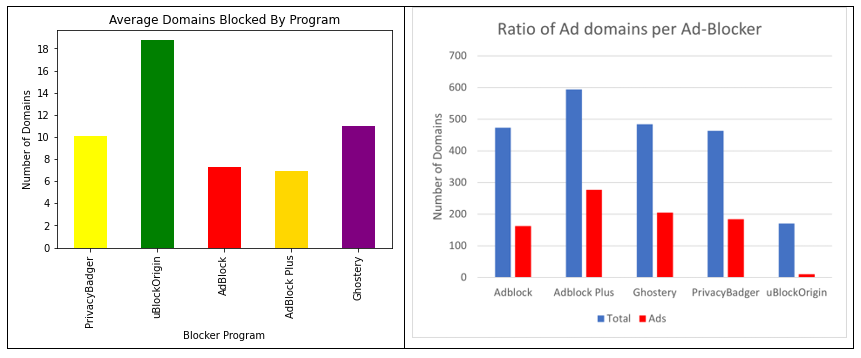
\includegraphics[scale = 0.75]{Edit3.png}
  \caption{ The leftmost graph(a) shows the average number of ad-domains reported by each adblocker. The rightmost graph(b) compares the total number of domains detected with a proxy to the number of those domains that are ads while each blocker was active.}
  \label{fig:graph1ab}
\end{figure}

The number of domains and ads blocked was first gathered from the blockers while in use and then gathered from proxy logs for comparison. The results of the first test found that uBlockOrigin detected and blocked the most domains with an average of 18 domains being blocked on each website. Ghostery and PrivacyBadger were the next best extensions with an average of 11 and 10 domains being blocked respectively. uBlockOrigin blocked around 50\% more domains on average than the other blockers as shown in figure 1a. Although PrivacyBadger is not marketed as an adblocker, it blocked more domains on average than Adblock and Adblock Plus. 
AdBlock and AdBlock Plus blocked the lowest number of domains with around seven being blocked on average and with mininal difference between the two blockers.  
 
The second test found that overall there were more domains and ads blocked by each blocker on average than reported by their icons as shown in figure 1b. Similarly to the first test, uBlockOrigin was found to block the most domains due to the fewest number of domains and ads being detected while it was active. With this test there was an inverse relationship with the blocker's performance and the number of domains detected and blocked. The fewer the amount of total domains and ads detected, the better the blocker. uBlockOrigin had less than 200 total domains to block while the other blockers had more than 400 total domains which indicates that uBlockOrigin performed 50\% better than the other blockers which is similar to the results of the first test. Adblock Plus had the most total domains active of nearly 600 and the most total ad-domains of around 280 which is slightly less than 50\%. In comparison, Adblock, Ghostery, and PrivacyBadger all had around 450-475 total domains active with around 160, 200, and 190 ad-domains detected respectively. Adblock and Ghostery had similar total domain counts while Ghostery had a greater proportion of ad-domains. PrivacyBadger fell somewhere inbetwen Ghostery and Adblock in terms of total domain and ad-domain counts.   

Overall, the results of both tests found that uBlockOrigin blocked around 50\% more domains than the other blockers individually. uBlockOrigin blocked the most domains on average in the first test and had significantly fewer ad-domains present in the second test which further testifies to its performance as an ad-blocker. PrivacyBadger and Ghostery had similar results in both tests. There was little difference between Adblock and Adblock Plus in the first test, but the second test showed a significant difference between the two with Adblock Plus having significantly more domains and ads being active. 

\section*{Future Work}
 Looking forward, we have identified a number of aspects of ad-blockers in addition to the ones we studied in this research project that could also be worth investigating. These consist of comparing the load time impacts of ad-blocking browser extensions with DNS-based services like Pi-Hole, exploring the effectiveness of combining ad-blocking browser extensions with DNS-based ones, and how running multiple ad-blockers of the same kind can affect their performances. We will next detail these ideas further in the following paragraphs, beginning with comparing the load time effects between ad-blocking browser extensions and DNS-based ad-blockers.

 In addition to how many ads are blocked, the effect of ad-blockers on the load times of internet browsers is also an important aspect to consider when determining which ad-blockers are truly the best. This, however, would prove to be a challenge to determine due to the natural variance in browser load times caused by changes in other variables such as network traffic, upload speed, and download speed. In order to effectively gauge the effects of ad-blockers on browser load times, a very stable network would be needed in which differences in load times are caused primarily by the ad-blockers, with any other variables being corrected for. It is worth noting, however, that the load-time effects of most of the ad-blocking extensions that we used in this research project have already been investigated in one of the studies detailed in the “Past Work” section \cite{10.1145/3091478.3091514}. DNS-based services like Pi-Hole, on the other hand, do not appear to have been studied as extensively, making their load-time performance compared to browser extensions a valuable opportunity for further study. Investigating this further could help to better identify which ad-blockers have the best performance which, in turn, could benefit consumers.
	
 Another topic of study that may be valuable to consumers would be the effectiveness of combining browser extension ad-blockers with DNS-based ones like Pi-Hole. Since these two kinds of ad-blocking software work differently, it may be possible that they could complement each other, resulting in a greater number of ad domains being blocked. This, however, does not appear to have been studied so far. Additionally, the effects of combining these two ad-blocker types on browser load times, to our knowledge, has also not been explored. Considering this, we believe that studying the effects of combining browser extensions and DNS-based services may offer valuable opportunities to further expand the knowledge base on ad-blocking software. Furthermore, if these two kinds of ad-blockers turn out to synergize well, it could pave the way to the development of more effective ad-blocking services or, at the very least least, it could help users make the most of the services that are currently available.
	
 Alongside investigating how different types of ad-blockers interact with each other, it also may be worth investigating how ad-blockers of the same type, either browser extensions or DNS-based services, could affect each other. Since much of the research on ad-blocker performance appears to consist of studying individual ad-blockers separately, this side of it remains somewhat unexplored. Additionally, it also may be somewhat common for users to make use of more than one ad-blocking browser extension at the same time. If so, studying how ad-blockers of the same type affect each other could be essential to fully understanding their effectiveness in the wild. This could be in terms of how many ads are blocked by each active ad-blocker, as well as how each ad-blocker affects the browser’s load times. Overall, a better understanding of the effects of using more than one ad-blocker of the same type could be beneficial to researchers by providing a more complete picture of ad-blocker effectiveness. Additionally, investigating this could also help consumers determine if using multiple ad-blockers is worthwhile.
	
 This idea, as well as the others discussed here, are far from the only open areas for further research into ad-blockers. We believe, however, that these ideas offer good starting points for filling in some of the missing pieces. Now, after looking at a few potential avenues for further research into ad-blockers, we will summarize the work that we performed in our own study alongside our key findings.

\section*{Conclusion}
In this study, we made use of the Stephen Black Hosts advertising domain list and a MITM Proxy server to compare the effectiveness of several popular ad-blocking extensions with Pi-Hole. These ad-blocking extensions consisted of AdBlock, AdBlock Plus, uBlock Origin, Ghostery, and Privacy Badger. To determine their effectiveness, we considered the number of domains that they claimed to block as well as the number of domains that still got through according to the MITM proxy. Then we used the Stephen Black Hosts list, the default filter list used by Pi-Hole, to identify ad domains that the extensions did not block but Pi-Hole would have blocked. We found that all of the ad-blockers tested blocked fewer ad domains from the list than Pi-Hole, with uBlock Origin blocking the most. Considering this, we conclude that using Pi-Hole will result in more ads being blocked than the ad-blocking extensions that we studied in this paper. Additionally, we have found that, among the ad-blocking browser extensions that we studied, uBlock Origin blocked the greatest number of ad domains identified by the Stephen Black Hosts list. This research could be further explored with additional browsers, combinations of extensions, and analysis of the blockers' resource usage to better gauge their effectiveness. 

\bibliographystyle{acm}
\bibliography{myBib}
\end{document}
